\documentclass{standalone}
\usepackage{tikz}
\usepackage{amsmath}
\usetikzlibrary{arrows.meta, positioning}

\begin{document}

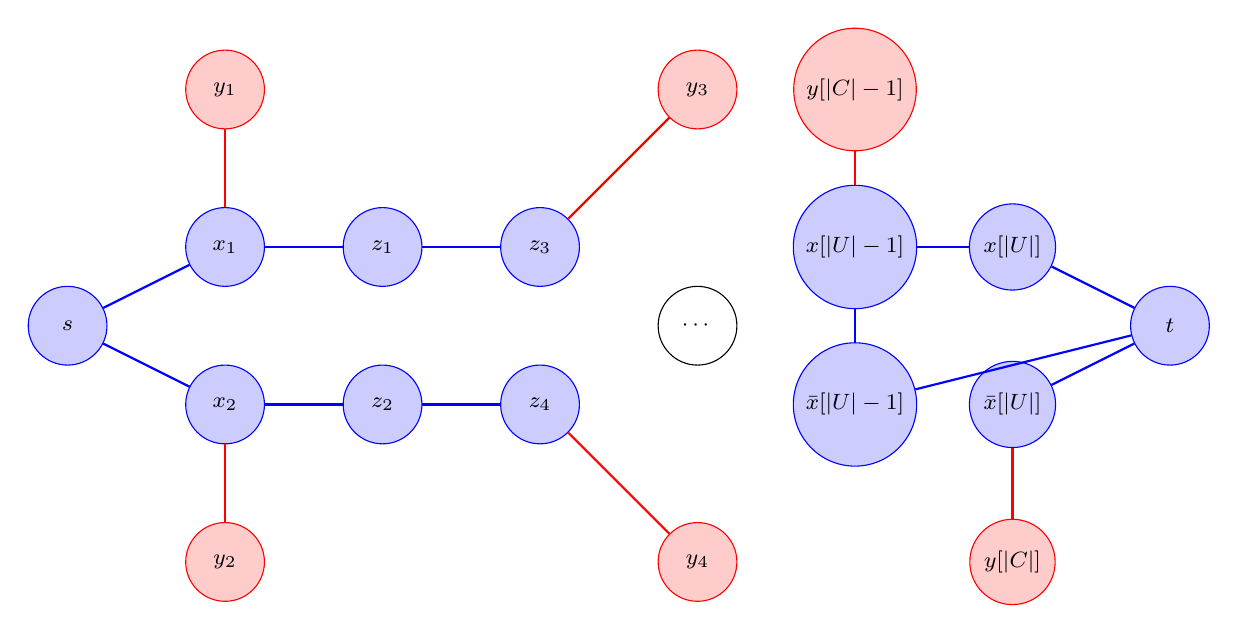
\begin{tikzpicture}[
    every node/.style={circle, draw, minimum size=1cm, font=\footnotesize},
    red node/.style={fill=red!20, draw=red},
    blue node/.style={fill=blue!20, draw=blue},
    blue edge/.style={blue, thick},
    red edge/.style={red, thick}
]

% Blue nodes and edges
\node[blue node] (s) at (0, 3) {$s$};
\node[blue node] (x1) at (2, 4) {$x_1$};
\node[blue node] (x2) at (2, 2) {$x_2$};
\node[blue node] (z1) at (4, 4) {$z_1$};
\node[blue node] (z2) at (4, 2) {$z_2$};
\node[blue node] (z3) at (6, 4) {$z_3$};
\node[blue node] (z4) at (6, 2) {$z_4$};

\node[blue node] (xU-1) at (10, 4) {$x[|U|-1]$};
\node[blue node] (xU) at (12, 4) {$x[|U|]$};
\node[blue node] (zU-1) at (10, 2) {$\bar{x}[|U|-1]$};
\node[blue node] (zU) at (12, 2) {$\bar{x}[|U|]$};

\node[blue node] (t) at (14, 3) {$t$};

% Red nodes and edges
\node[red node] (y1) at (2, 6) {$y_1$};
\node[red node] (y2) at (2, 0) {$y_2$};
\node[red node] (y3) at (8, 6) {$y_3$};
\node[red node] (y4) at (8, 0) {$y_4$};

\node[red node] (yC-1) at (10, 6) {$y[|C|-1]$};
\node[red node] (yC) at (12, 0) {$y[|C|]$};

% Blue edges
\draw[blue edge] (s) -- (x1);
\draw[blue edge] (s) -- (x2);
\draw[blue edge] (x1) -- (z1);
\draw[blue edge] (x2) -- (z2);
\draw[blue edge] (z1) -- (z3);
\draw[blue edge] (z2) -- (z4);

\draw[blue edge] (xU-1) -- (xU);
\draw[blue edge] (xU-1) -- (zU-1);
\draw[blue edge] (xU) -- (t);
\draw[blue edge] (zU-1) -- (t);
\draw[blue edge] (zU) -- (t);

% Red edges
\draw[red edge] (y1) -- (x1);
\draw[red edge] (y2) -- (x2);
\draw[red edge] (y3) -- (z3);
\draw[red edge] (y4) -- (z4);

\draw[red edge] (yC-1) -- (xU-1);
\draw[red edge] (yC) -- (zU);

% Dotted line for ellipsis
\node at (8, 3) {$\cdots$};

\end{tikzpicture}

\end{document}